After the high level components were designed, the user stories helped create a more detailed view of them. At that point of
time the project focused on sprint one, which meant focusing on evaluating individuals over a network.
User stories helped identify how user was going to approach the framework hence it was able to create components with known
input and return parameters as seen in figure \ref{fig:firstSprint}


\begin{figure}[htp]
\centering
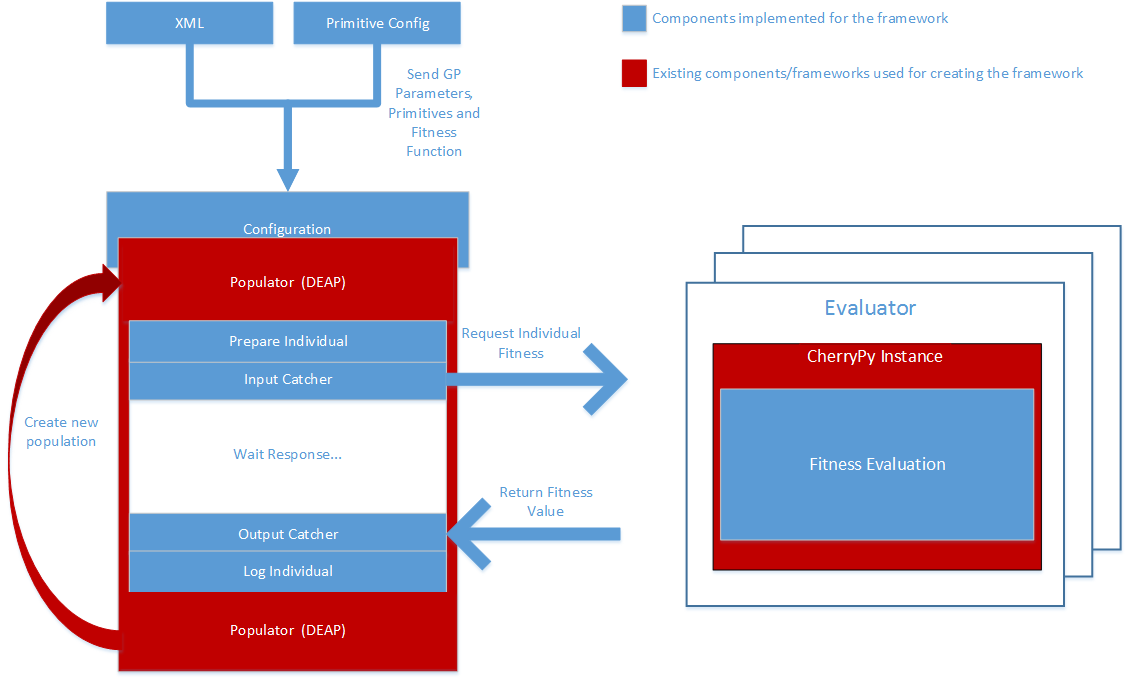
\includegraphics[scale=0.6]{Figures/FirstSprint.png}
\caption{Lower level component diagram showing the functionality and usage of each class/component}
\label{fig:firstSprint}
\end{figure}


Even though Python2.7, unlike Python3.3 is a semi object language, for better use of software engineering practices and better ordering of the project,
objects were used to represent the different components. The diverse capabilities of python and large set of libraries helped design a complex framework with reliable simple architecture. The prime design principle followed
was loose coupling and high cohesion since it allows modularity and helps for the management of a complex systems. This design helped insert the technologies that are used at the correct
places. Proceeding in a top-down manner helped us clearly identify the components.



